\documentclass{article}

\usepackage[english]{babel}
\usepackage{csquotes}
\usepackage[letterpaper,top=2cm,bottom=2cm,left=3cm,right=3cm,marginparwidth=1.75cm]{geometry}

\newcommand{\currentversion}{2.8}

\usepackage{amsmath}
\usepackage{graphicx}
\usepackage{biblatex}
\usepackage{float}
\usepackage{multirow}
\usepackage[colorlinks=true, allcolors=blue]{hyperref}
\addbibresource{references.bib}
\title{
\includegraphics[width=0.8\textwidth]{MINI.png} \\ Project of Application for Piano Music Generation \\ by Artificial Intelligence Algorithms \\ [0.35em]\large Laboratory No. 2, \\ Version \currentversion }
\author{}
\date{}

\begin{document}
\maketitle
\begin{center}
    \normalsize\textbf{Authors:}
    \vskip10pt
    \Large{Szymon Górski} \\
    \large{Index No. 298796}
    \vskip10pt
    \Large{Weronika Piotrowska} \\
    \large{Index No. 305793}
    \vskip10pt
    \Large{Marcin Wojnarowski} \\
    \large{Index No. 303880}
    \vskip50pt
    \normalsize\textbf{Thesis Supervisor:}
    \vskip10pt
    \Large{Jerzy Balicki} \\
    \large{DSc, Associate Professor}
    \vfill
    \large{Warsaw, 2022}
\end{center}

\newpage
\begin{abstract}
    This document outlines the bachelor thesis project for the last semester of Computer Science and Information Systems at the Faculty of Mathematics and Information Science Warsaw University of Technology. Project assumptions and requirements are presented regarding the concept of generation music with Machine Learning techniques. Users can interact with the models through a user interface.

    \hfill


    \textbf{Sections 1-5 are a part of \textit{Deliverable 1}.}
\end{abstract}

\vskip50pt
\section*{History of changes}
\begin{center}
    \begin{tabular}{ |p{0.07\textwidth} | p{0.1\textwidth} | p{0.5\textwidth} | p{0.21\textwidth}| }
        \hline
        Version         & Date       & Description                                                          & Author              \\
        \hline
        1               & 15.10.2022 & Initial creation of the document.                                    & Weronika Piotrowska \\
        \hline
        1.1             & 15.10.2022 & Added vocabulary, executive summary and non-functional requirements  & Weronika Piotrowska \\
        \hline
        1.2             & 15.10.2022 & Added non-functional requirements.                                   & Weronika Piotrowska \\
        \hline
        1.3             & 16.10.2022 & Added user stories and functional requirements.                      & Marcin Wojnarowski  \\
        \hline
        1.4             & 16.10.2022 & Added document abstract.                                             & Marcin Wojnarowski  \\
        \hline
        1.5             & 16.10.2022 & Added SWOT analysis.                                                 & Szymon Górski       \\
        \hline
        1.6             & 17.10.2022 & Added project schedule.                                              & Szymon Górski       \\
        \hline
        1.7             & 18.10.2022 & Added use-case descriptions.                                         & Marcin Wojnarowski  \\
        \hline
        1.8             & 18.10.2022 & Added motivation and goal description                                & Weronika Piotrowska \\
        \hline
        1.9             & 18.10.2022 & Added Gantt diagram.                                                 & Szymon Górski       \\
        \hline
        1.10            & 18.10.2022 & Added work division.                                                 & Szymon Górski       \\
        \hline
        1.11            & 19.10.2022 & Added use case diagram.                                              & Marcin Wojnarowski  \\
        \hline

        2.0             & 09.11.2022 & Initial creation of the document, basing on Laboratory 1 Deliverable & Weronika Piotrowska \\
        \hline

        2.1             & 10.11.2022 & Added dataset description                                            & Weronika Piotrowska \\
        \hline

        2.2             & 12.11.2022 & Added System architecture and models design                          & Szymon Górski       \\
        \hline

        2.3             & 12.11.2022 & Added Main Components diagrams                                       & Weronika Piotrowska \\
        \hline
        2.4             & 12.11.2022 & Added Technology Selection section                                   & Marcin Wojnarowski  \\
        \hline

        2.5             & 13.11.2022 & Added External Interfaces section                                    & Marcin Wojnarowski  \\
        \hline
        2.6             & 13.11.2022 & Added Communication                                                  & Szymon Górski       \\
        \hline

        2.7             & 14.11.2022 & Added Model Selection description                                    & Weronika Piotrowska \\
        \hline
        \currentversion & 14.11.2022 & Added GUI vision section and OpenAPI attachment                      & Marcin Wojnarowski  \\
        \hline
    \end{tabular}
\end{center}

\newpage


\tableofcontents
\newpage

\section{Introduction}
\subsection{Motivation}
Even though Artificial Intelligence is known for its various applications in majority of Information Sciences, the topic of music processing is not yet widely developed. Basing on existing solutions for image and video processing, we will implement and put in comparison three generative models. The motivation behind this project is to explore possible ways of music generation with the use of Machine Learning and to give this possibility to others by creating an user-friendly application that will show the effects of our work.

\subsection{Goals}

The aim of work is implementation and comparison of algorithms that can be used for music generation, as well as building an application, which will show the effects. We propose the following specification in order to achieve this goal. The specification includes descriptions of executive summary, functional requirements, along user stories and use cases, and non-functional requirements divided into URPS categories. To achieve our goal, we have designed a schedule of work presented in Gantt's diagram and division of work among project members. Finally, we present risk analysis prepared in a form of SWOT diagram.

\noindent
Optional goal is to generate a piece which is non-distinguishable from the original dataset. This issue, however, is mostly based on a subjective impression of an individual and is too complicated to be evaluated by a computer and will not be focused on in this project.

\section{Vocabulary} \label{vocab}
\textbf{Artificial Intelligence} - The capacity of computers or other machines to exhibit or simulate intelligent behavior; the field of study concerned with this. Abbreviated AI. \cite{AI_OED}

\vskip5pt \noindent
\textbf{Machine Learning} - Machine learning is a branch of artificial intelligence (AI) and computer science which focuses on the use of data and algorithms to imitate the way that humans learn, gradually improving its accuracy. \cite{ML_IBM}

\vskip5pt \noindent
\textbf{Neural Network} - algorithmic structure, which is the core of deep learning algorithms; Their name and structure are inspired by the human brain, mimicking the way that biological neurons signal to one another. \cite{NN_IBM}

\vskip5pt \noindent
\textbf{LSTM} - Long Short-Term Memory; an artificial neural network used in the fields of artificial intelligence and deep learning. Unlike standard feedforward neural networks, LSTM has feedback connections. Such network can process not only single data points, but also entire sequences of data (such as recordings). \cite{LSTM}

\vskip5pt \noindent
\textbf{CNN} - Convolutional Neural Network; a neural network architecture using convolutional layers, which is advantageous in case of image processing. \cite{CNN}

\vskip5pt \noindent
\textbf{Markov Chain} - a stochastic model describing a sequence of possible events in which the probability of each event depends only on the state attained in the previous event. In this case, it will be referred to predicting next piano chords based on given number of previous chords. \cite{Markov}

\vskip5pt \noindent
\textbf{MIDI} - Musical Instrument Digital Interface. Standard file format describing notes being played at a given instant and how loud they are. As opposed to audio files, MIDI does not store actual audio.


\vskip5pt \noindent
\textbf{Acceptance criteria} - A set of conditions the system has to fulfill to be accepted by the user story agent (user/customer/admin). Once those are fulfilled, the user story can be considered as done and closed. Abbreviated AC.


\section{Specification}

\subsection{Executive summary}

The application will enable a user to upload their own audio files in MIDI format to train a selected model. Afterwards the user is able to generate a music sample generated by the model trained on the previously provided input. The program will base on Machine Learning algorithms, including LSTM and Convolutional Networks. The aim of the application is to provide an educational presentation of the performance of implemented models based on the given data.

\subsection{Functional requirements}

To begin, a strict set of requirements has to be defined. Most requirements are expressed as User Stories but we also provide a general list of requirements. A clear definition of requirements is crucial as it will be our main reference of our progress and will ensure that our system is complete and cohesive. The system will be split into three components, each with a separate responsibility: \textit{server}, \textit{client}, and \textit{model}.

\subsubsection{User stories}

\newcommand{\AC}{\subitem AC. }

\textbf{\large Model:}

Below are stories related to the \textit{model} component.

\begin{enumerate}
    \item
          As a user, I want to be able to process MIDI files.
          \AC Model component is able to read MIDI files and store them in a custom structure.

    \item
          As a user, I want to be able to train the a model with given input.
          \AC A function is exposed for each model which accepts input and trains the model.

    \item
          As an admin, I want to be able to track my model's performance.
          \AC Model saves training progress.
          \AC Training progress can be accessed and processed further.

    \item
          As an admin, I want to be able to test my model's performance.
          \AC Model can estimate its performance in a quantitative manner.

    \item
          As a user, I want to be able to save a trained model.
          \AC Model can be saved to a persistent medium.
          \AC Saved model is easily exportable to a different computer.

    \item
          As a user, I want to be able to load a saved model.
          \AC Model can be loaded from a persistent medium.
          \AC Model's performance is retained when loading the model.

    \item
          As a user, I want to be able to generate new music.
          \AC Model generates MIDI files based on a given seed.
\end{enumerate}

\newpage
\textbf{\large Client \& Server:}

Below are stories related to the \textit{client} and \textit{server} component. User stories here describe the user perspective of interaction with the system however, these also entail some backend work as well.

\begin{enumerate}
    \item
          As a user, I want to be able to open a web page containing an app interface.
          \AC Web page displays some greeting interface.

    \item
          As a user, I want to be able to choose the target model.
          \AC UI presents a select field allowing to choose a model.
          \AC Once the choice has been made user can go to the next stage.

    \item
          As a user, I want to be able to pick either a pre-trained model or to train one myself.
          \AC User is presented with a choice between pre-trained and train yourself.
          \AC Once the choice has been made user can go to the next stage.

    \item
          As a user, I want to be able to upload MIDI files if I chose to train the model myself.
          \AC UI presents an option to choose a folder with MIDI files in it.
          \AC Files can be drag\&dropped for upload.
          \AC Files are sent to the backend server.

    \item
          As a user, I want to be able see the training progress.
          \AC A live-updating chart shows the training model performance.

    \item
          As a user, I want to be able to interrupt the training process so that I can start using the model immediately.
          \AC By pressing the interrupt button the training process stops.
          \AC User can move to the generation stage.

    \item
          As a user, I want to be able to generate music by providing a simple seed.
          \AC User can provide a music seed to start the generation process.
          \AC User can choose generated music length in seconds.
          \AC Generated music is saved to MIDI on the computer.
\end{enumerate}

\newpage
\subsubsection{Use-case descriptions}

To be more specific, a list of core functional requirements as use cases is presented below.

\begin{center}
    \begin{tabular}{ |p{0.11\textwidth}|p{0.15\textwidth}|p{0.25\textwidth}|p{0.37\textwidth}| }
        \hline
        Actor     & Name                & Description                                 & System response                                                                                                                                                                                                   \\
        \hline
        \multicolumn{4}{|l|}{\textbf{Models}}                                                                                                                                                                                                                                                             \\
        \hline
        Developer & Model training      & Training a model with a given dataset       & Module creates a previously defined model and trains it with progress saving.                                                                                                                                     \\
        \hline
        Developer & Model evaluation    & Evaluating a model against given data       & Module creates loads a previously trained model and evaluates its performance after which the results are presented.                                                                                              \\
        \hline
        Developer & Music generation    & Generating music given a starting seed.     & Model accepts a seed and generates a sequence. This sequence is saved to a MIDI file.                                                                                                                             \\
        \hline
        Developer & MIDI parsing        & Being able to read and write MIDI files.    & System can read MIDI files and process to our needs. System can create MIDI files from model outputs.                                                                                                             \\
        \hline
        \multicolumn{4}{|l|}{\textbf{Server}}                                                                                                                                                                                                                                                             \\
        \hline
        Developer & Model integration   & Server and model components are integrated. & Server component can query models for various things (training, evaluation, generation) and receives back responses.                                                                                              \\
        \hline
        Developer & API                 & Server exposes an API.                      & Client receives responses from the server regarding queries and commands.                                                                                                                                         \\
        \hline
        Developer & File streaming      & Streaming files from and to a client.       & Client can download a file from the server. Server receives streamed files from the client.                                                                                                                       \\
        \hline
        \multicolumn{4}{|l|}{\textbf{Client}}                                                                                                                                                                                                                                                             \\
        \hline
        User      & Model configuration & Configuration of target model               & Buttons and switches are shown on the UI to allow for choosing the model and training status (pre-trained/new).                                                                                                   \\
        \hline
        User      & File upload         & Uploading local files to the server         & Application accepts MIDI files to be uploaded. Files are sent to the backend server as the input dataset.                                                                                                         \\
        \hline
        User      & Model training      & Training a selected model                   & Server communicates with the models in order to train them. Server streams training progress back to the client. Client displays training progress in the form of live-updating charts and/or standalone scalars. \\
        \hline
        User      & Music generation    & Using a model to generate music             & Server communicates with the models in order to generate music sequences. Server sends a MIDI file back to the client. Client downloads the generated MIDI file.                                                  \\
        \hline
    \end{tabular}
\end{center}

\newpage
\subsubsection{Use case diagram}

Since most of the functionality will be on the side of designing and creating models which is behind the scenes, the use case diagram can be neatly summarized to the main features.


\begin{figure}[H]
    \centering
    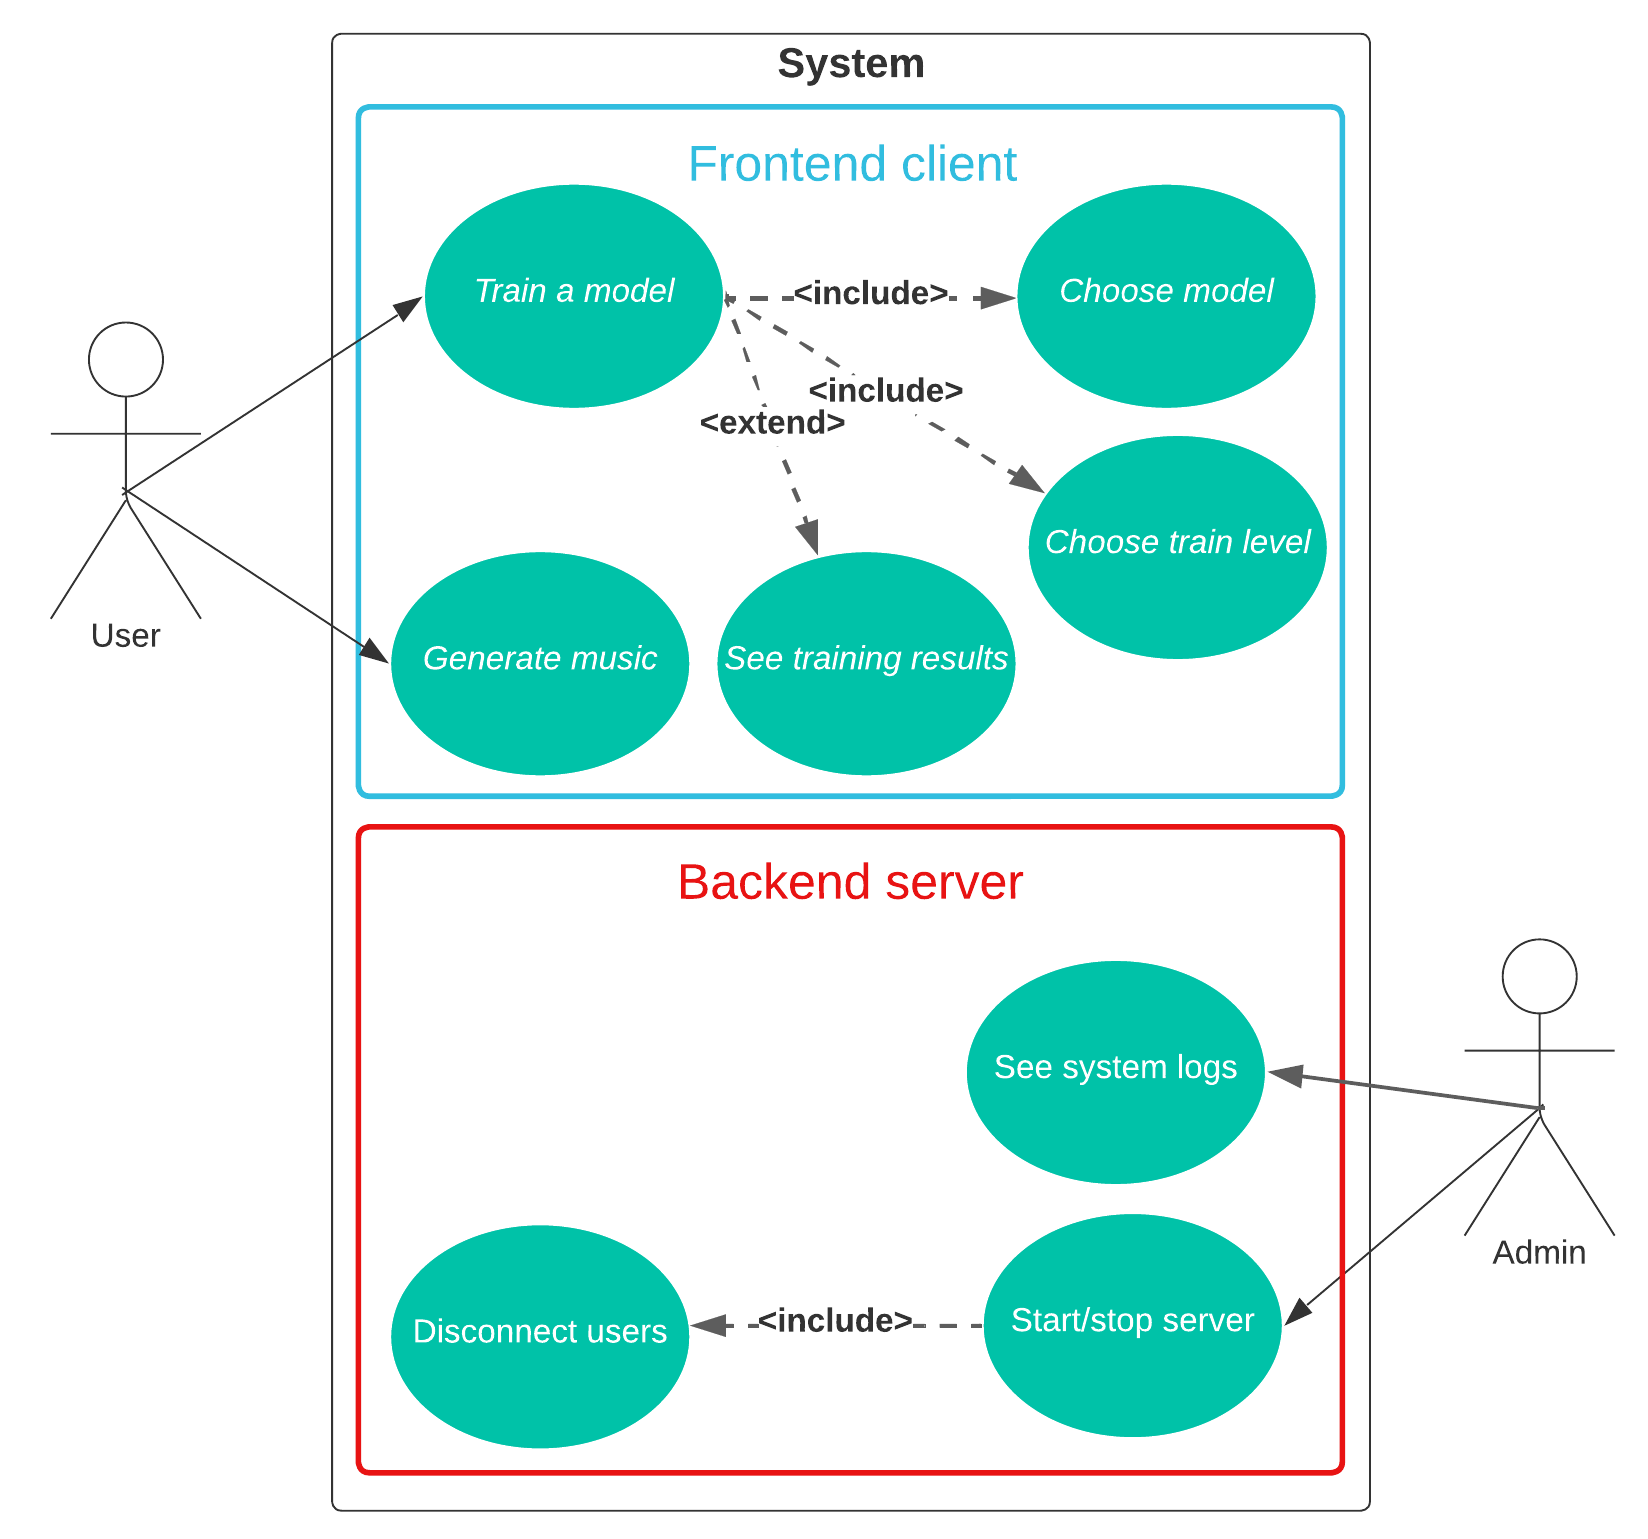
\includegraphics[width=0.7\textwidth]{use_case_diagram.png}
    \caption{Use case diagram for the user and admin interacting with the system.}
    \label{fig:use-case-diagram}
\end{figure}

\subsection{Non-functional requirements}
Below are examples of non-functional requirements grouped into individual URPS (Usability, Reliability, Performance, Supportability) categories:

\begin{center}
    \begin{tabular}{ |p{0.15\linewidth}|p{0.13\linewidth}|p{0.6\linewidth}| }
        \hline
        Requirements area                 & Requirement No. & Description                                                                                                                                                              \\
        \hline
        \multirow{3}{1em}{Usability}      & 1               &
        The application window must fit into a single screen of standard size (minimum 1920 x 1080 px)                                                                                                                                 \\
        \cline{2-3}
                                          & 2               & The application must be clear and legible, with font size not smaller than 10. All images and graphs displayed in the application must not be compressed in the runtime. \\
        \cline{2-3}
                                          & 3               & File upload must be working regardless of operating system.                                                                                                              \\
        \hline
        \multirow{1}{4em}{Reliability}    & 4               & The application must be available at least 99\% of the time, with exception of server service breaks.                                                                    \\
        \hline
        \multirow{2}{4em}{Performance}    & 5               & The application should provide exchange of information between user and server in no longer than 3 seconds.                                                              \\
        \cline{2-3}
                                          & 6               & When training a model, the application should update on its progress.                                                                                                    \\
        \hline
        \multirow{2}{4em}{Supportability} & 7               & The application must be backwards compatible with all of its components.                                                                                                 \\
        \cline{2-3}
                                          & 8               & In case of any exception, the application should provide a detailed information to the user.                                                                             \\
        \hline
    \end{tabular}
\end{center}

\section{Project schedule}
\subsection{Scope of work}
The following table presents division of the project into parts and tasks with their respective time necessary to finish each assignment. Six main parts of the project were separated due to their subject.

\begin{center}
    \begin{tabular}{ |p{0.13\linewidth}|p{0.55\linewidth}|p{0.20\linewidth}| }
        \hline
        Part No.                                                                & Task                                                 & Duration (weeks) \\
        \hline
        \multicolumn{2}{|l|}{\textbf{1. Project preparation}}                   & \textbf{10}                                                             \\
        \hline
        1.1                                                                     & Research and study on the thesis' topic              & 4.5              \\
        \hline
        1.2                                                                     & Research and study on available algorithms and tools & 4.5              \\
        \hline
        1.3                                                                     & Choice of the AI algorithms and the technology stack & 1                \\
        \hline
        \multicolumn{2}{|l|}{\textbf{2. Data management}}                       & \textbf{6}                                                              \\
        \hline
        2.1                                                                     & Research of available datasets                       & 3                \\
        \hline
        2.2                                                                     & Choice of datasets to be included and accessing them & 1                \\
        \hline
        2.3                                                                     & Implementation of MIDI transcription module          & 2                \\
        \hline
        \multicolumn{2}{|l|}{\textbf{3. 1st model development}}                 & \textbf{5}                                                              \\
        \hline
        3.1                                                                     & Model implementation                                 & 3                \\
        \hline
        3.2                                                                     & Model evaluation                                     & 1                \\
        \hline
        3.3                                                                     & Model testing and tuning                             & 1                \\
        \hline
        \multicolumn{2}{|l|}{\textbf{4. 2nd model development}}                 & \textbf{5}                                                              \\
        \hline
        4.1                                                                     & Model implementation                                 & 3                \\
        \hline
        4.2                                                                     & Model evaluation                                     & 1                \\
        \hline
        4.3                                                                     & Model testing and tuning                             & 1                \\
        \hline
        \multicolumn{2}{|l|}{\textbf{5. Client-server application development}} & \textbf{4}                                                              \\
        \hline
        5.1                                                                     & Client-server application establishment              & 2                \\
        \hline
        5.2                                                                     & Graphic User Interface design and implementation     & 1                \\
        \hline
        5.3                                                                     & Application integration with both AI models          & 1                \\
        \hline
        \multicolumn{2}{|l|}{\textbf{6. Testing}}                               & \textbf{4}                                                              \\
        \hline
        6.1                                                                     & Unit testing                                         & 1                \\
        \hline
        6.2                                                                     & Integration testing                                  & 1                \\
        \hline
        6.3                                                                     & System testing                                       & 1                \\
        \hline
        6.4                                                                     & Efficiency and quality comparison of both AI models  & 1                \\
        \hline
        6.5                                                                     & Final corrections and system review                  & 1                \\
        \hline
    \end{tabular}
\end{center}

\newpage
\subsection{Gantt diagram}

The following pictures represent a Gantt diagram locating assignments in a timetable. It also represents dependencies between particular tasks presented above.

\begin{center}
    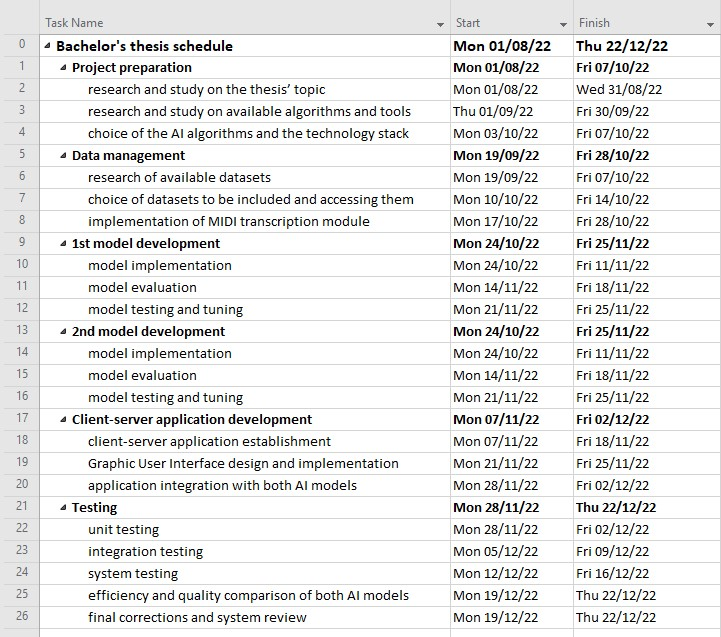
\includegraphics[width=0.7\textwidth]{Gantt_1.jpg} \\
    \textit{Part 1:} List of tasks with their respective dates of staring and finishing
    \vskip10pt \noindent
    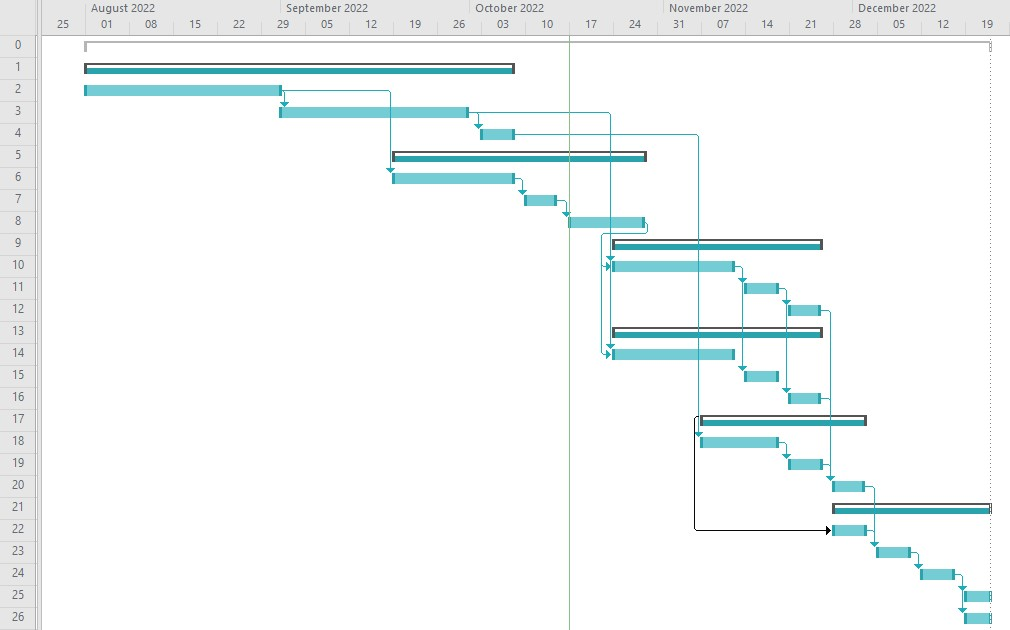
\includegraphics[width=1\textwidth]{Gantt_2.jpg} \\
    \textit{Part 2:} Diagram of tasks and their dependencies against time \\ (as of 17 October 2022, represented by a green line)
\end{center}

\subsection{Work division}
The following table shows the distribution of tasks among the authors. The division was designed to provide equal allocation of work as well as its continuity of performance. Some work should be or already have been done by all together - these assignments were presented under 'collective tasks'.

\begin{center}
    \begin{tabular}{ |p{0.23\linewidth}|p{0.67\linewidth}| }
        \hline
        Author                                           & Tasks         \\
        \hline
        \multirow{3.75}{10em}{\textit{Collective tasks}} &
        \begin{itemize}
            \item [1.] Project preparation
            \item [2.1.] Research of available datasets
            \item [6.5.] Final corrections and system review
        \end{itemize}                  \\
        \hline
        \multirow{3.75}{10em}{Szymon Górski}             &
        \begin{itemize}
            \item [2.2.] Choice of datasets to be included and accessing them
            \item [2.3.] Implementation of MIDI transcription module
            \item [4.] 2nd model development
            \item [5.2.] Graphic User Interface design and implementation
            \item [6.1.] Unit testing
        \end{itemize} \\
        \hline
        \multirow{3.75}{10em}{Weronika Piotrkowska}      &
        \begin{itemize}
            \item [3.] 1st model development
            \item [5.2.] Graphic User Interface design and implementation
            \item [5.3.] Application integration with both AI models
            \item [6.3.] System testing
            \item [6.4.] Efficiency and quality comparison of both AI models
        \end{itemize}  \\
        \hline
        \multirow{3.75}{10em}{Marcin Wojnarowski}        &
        \begin{itemize}
            \item [4.] 2nd model development
            \item [5.1.] Client-server application establishment
            \item [5.3.] Application integration with both AI models
            \item [6.2.] Integration testing
        \end{itemize}          \\
        \hline
    \end{tabular}
\end{center}

\newpage
\section{Risk analysis}
A risk analysis of the project was done using the 'SWOT' methodology. The result is presented in the following table.

\begin{center}
    \begin{tabular}{ |p{0.15\linewidth}|p{0.365\linewidth}|p{0.365\linewidth}| }
        \hline
        \multicolumn{1}{|c|}{\textbf{SWOT}}                                                                                                              & \multicolumn{1}{|c|}{HELPFUL}                 & \multicolumn{1}{|c|}{HARMFUL}              \\
        \hline
                                                                                                                                                         &                                               &                                            \\
        \multicolumn{1}{|c|}{INTERNAL}                                                                                                                   & \multicolumn{1}{|c|}{\textbf{Strengths:}}     & \multicolumn{1}{|c|}{\textbf{Weaknesses:}} \\
                                                                                                                                                         &
        \begin{enumerate}
            \item One of the authors has experience in developing music-generating AI systems,
            \item Possibility of consultation of solution design with people experienced in the field of music generation and AI (e.g., Project Supervisor),
            \item Extensive coverage of capabilities of used tools both in documentations and on the Internet,
            \item Multiple sets with MIDI files available in free domain,
            \item Good communication skills and motivation of all authors.
        \end{enumerate} &
        \begin{enumerate}
            \item Short period of time dedicated to developing core functions, while some learning algorithms may require significant amount of time to perform its tasks,
            \item Quality of results cannot be predicted straightforwardly,
            \item Impossibility of generating a MIDI set by one's own - the project depends on works by external authors,
            \item Large size, quality, and feature differences among different MIDI sets.
        \end{enumerate}                                                                                 \\
        \hline
                                                                                                                                                         &                                               &                                            \\
        \multicolumn{1}{|c|}{EXTERNAL}                                                                                                                   & \multicolumn{1}{|c|}{\textbf{Opportunities:}} & \multicolumn{1}{|c|}{\textbf{Threats:}}    \\
                                                                                                                                                         &
        \begin{enumerate}
            \item Raise of competence in the field of Artificial Intelligence,
            \item Possibility of further development of the project (e.g., as a master's thesis),
            \item Possibility of publishing the project on the Internet and gaining users (similarly to other AI projects e.g., DALL-E and its derivatives).
        \end{enumerate} &
        \begin{enumerate}
            \item Simultaneous completion of multiple projects throughout the semester,
            \item Some functionalities regarding learning algorithms may prone to fail or take too long to complete due to unsatisfactory (substandard) parameters of a user's PC,
            \item Consecutive development of the solution may happen in different periods than defined in the university's curriculum due to the need to focus on AI algorithms.
        \end{enumerate}                                                                         \\
        \hline
    \end{tabular}
\end{center}



\section{Initial dataset description}
\subsection{Overview}
The initial dataset consists of nearly 200 piano pieces written by Johann Sebastian Bach. The files are in MIDI format, obtained from an open-source page \hyperlink{https://www.bachcentral.com/midiindexcomplete.html}{Bach Central}. MIDI format is known for various advantages when it comes to audio processing; not only is it easily converted to numerical values, but also it does not initially define the instrument the music should be played on. It is very beneficial for the project, since Bach did not only write piano pieces, but using MIDI all files can be interpreted as such.

Johann Sebastian Bach is known for devoting attention to structure of his compositions. His compositions often contain the same, transformed structures and mathematical concepts. For example, the piece \textit{Crab Canon} from \textit{The Musical Offering} can be written and read from a Möbius strip.\cite{Mobius} Therefore, we believe that the compositions tied to mathematics could be replicable by artificial intelligence.

\subsection{Encoding} \label{encoding}

The following image illustrates a sample MIDI file in \hyperlink{http://www.midieditor.org/}{MidiEditor} program.

\begin{center}
    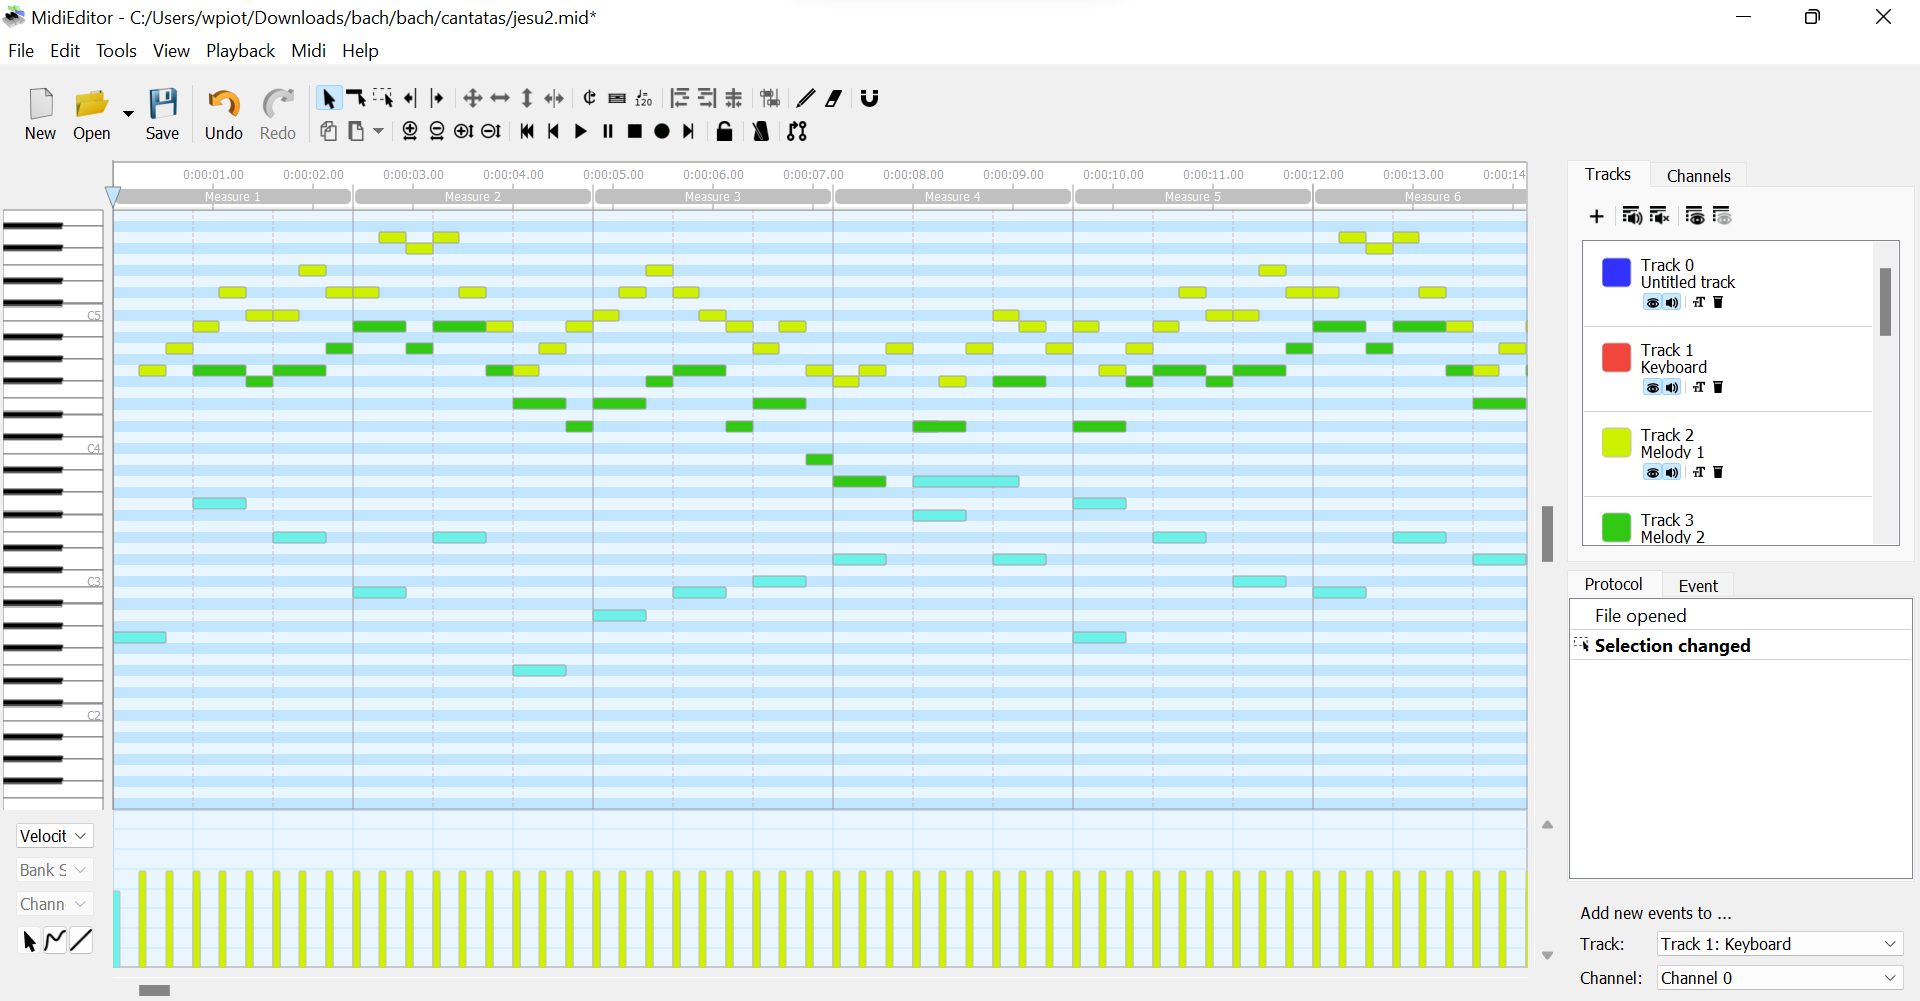
\includegraphics[width=1\textwidth]{midi_sample.png} \\
    Cantata \textit{Jesu, meine Freunde} by Johann Sebastian Bach showed in MidiEditor.
    \vskip10pt \noindent
\end{center}

The simplest case of interpreting a MIDI file is to look at it as a matrix of notes and time units. When entry of the matrix is 1 in i-th row and j-th column, this means that the i-th note is played in j-th time unit. Alongside of that, the file contains different tracks that are played. Since tracks are not usually consistent with each other, we have decided to split the data such that it would represent tracks. We achieved it by adding a third dimension to the matrix, turning it into a tensor.

This encoding was chosen because it resembles an image encoding in machine learning, where the tensor contains information about the place of a pixel (width and height of an image) and the color channel (R, G, B). Adjusting this approach to music files, we treat each track as a different color channel. In this way, channels are independent, but are processed together with other channels, giving us a consistent result.

\section{Model selection} \label{models}
% we can edit it if we change our mids ig

The client will see three different models and their performance on the initial dataset. The client can modify this dataset, train the chosen model again and see example of generated files. This section is devoted to short description of chosen Machine Learning models and reasons why they are suitable for our problem.

\subsection{Hidden Markov Model}

Similarly to Markov Chains (mentioned in Section \ref{vocab}), Hidden Markov Model bases on measuring probability of next state in a sequence. By implementing HMM, we will train the probability matrix using only linear transformations. To implement the model, we can use \href{https://hmmlearn.readthedocs.io/en/latest/tutorial.html#available-models}{hmmlearn} library in Python.

It is worth to notice that HMM is not a Neural Network. However, it is widely used in pattern and speech recognition. There were attempts to use it for music generation \cite{Li_2019} which yielded satisfactory results. Thus, we believe implementing this model can be a good starting point for the task.

\subsection{LSTM}

LSTM Networks, as mentioned in Section \ref{vocab}, are recurrent Neural Networks, which means the model will use outputs that it has produced to compute next element in a sequence. LSTMs use \textit{gating mechanisms} to control the memorizing process and as a result avoid the problem of forgetting long-term dependences in a sequence.

LSTMs have been widely used in all Machine Learning problems and has outpreformed Recurrent Neural Networks in classyfing and predicting time series. There are approaches to music generation using LSTMs \cite{lstm_arxiv}, but it is not a common practice to use these models.

\subsection{GAN}

GANs (mentioned is Section \ref{vocab}) are generative models widely used in image processing. A GAN consists of a Generator - a model that generates new data samples and a Discriminator - a model that discriminates against fake and real data. While training a GAN, we train generator and discriminator simultaneously, making them "compete" against each other. This architecture is a baseline of today's image generating models.

In section \ref{encoding} we have compared our encoding to an image encoding. Therefore, we believe that using GAN in music generation could bring results as good as it brings with image generation.
% \subsection{Stable Diffusion}

\section{System architecture}
The application consists of three following modules. The modules are designed so that replacing one module will not affect other modules.

\subsection{Models}
This module consists of pre-trained models (Section \ref{models}), which can be also trained on datasets provided by the client. The main responsibilities of this module are:
\begin{itemize}
    \item Train and evaluate chosen model according to user's input
    \item Generate samples of music
    \item Change the training dataset to one provided by the user
    \item Adjust user's data to match model's input (Section \ref{encoding})
\end{itemize}

\subsection{Backend server}
The role of a backend server is to integrate between user and model. The main responsibilities of this module are:
\begin{itemize}
    \item Query models for training, evaluation and generation
    \item Answer client's queries
    \item Stream files from and to a client
    \item Save system logs
    \item Assert correct format of streamed files
\end{itemize}

\subsection{Frontend}
Frontend module will provide a GUI, which will allow the user to use the application. Its main responsibilities are:
\begin{itemize}
    \item Allow user to select, configure and train a model
    \item Allow user to upload own training dataset
    \item Allow user to download generated files
    \item Inform about model's training progress
    \item Allow user to interrupt the training
    \item Display error messages
\end{itemize}

\section{Modules design}
\subsection{Layers}
We divide the application into two layers
\begin{itemize}
    \item Backend
    \item Frontend
\end{itemize}
The backend layer is responsible for implementing Model and API components. The frontend layer contains web application that will interact with the user.

\subsection{Dependencies, class diagram}
Since the point of our application is to build and test Machine Learning models, there is no complicated dependencies between the classes. The relationship between the classes can be described using the following conceptual class diagram:

\begin{figure}[H]
    \centering
    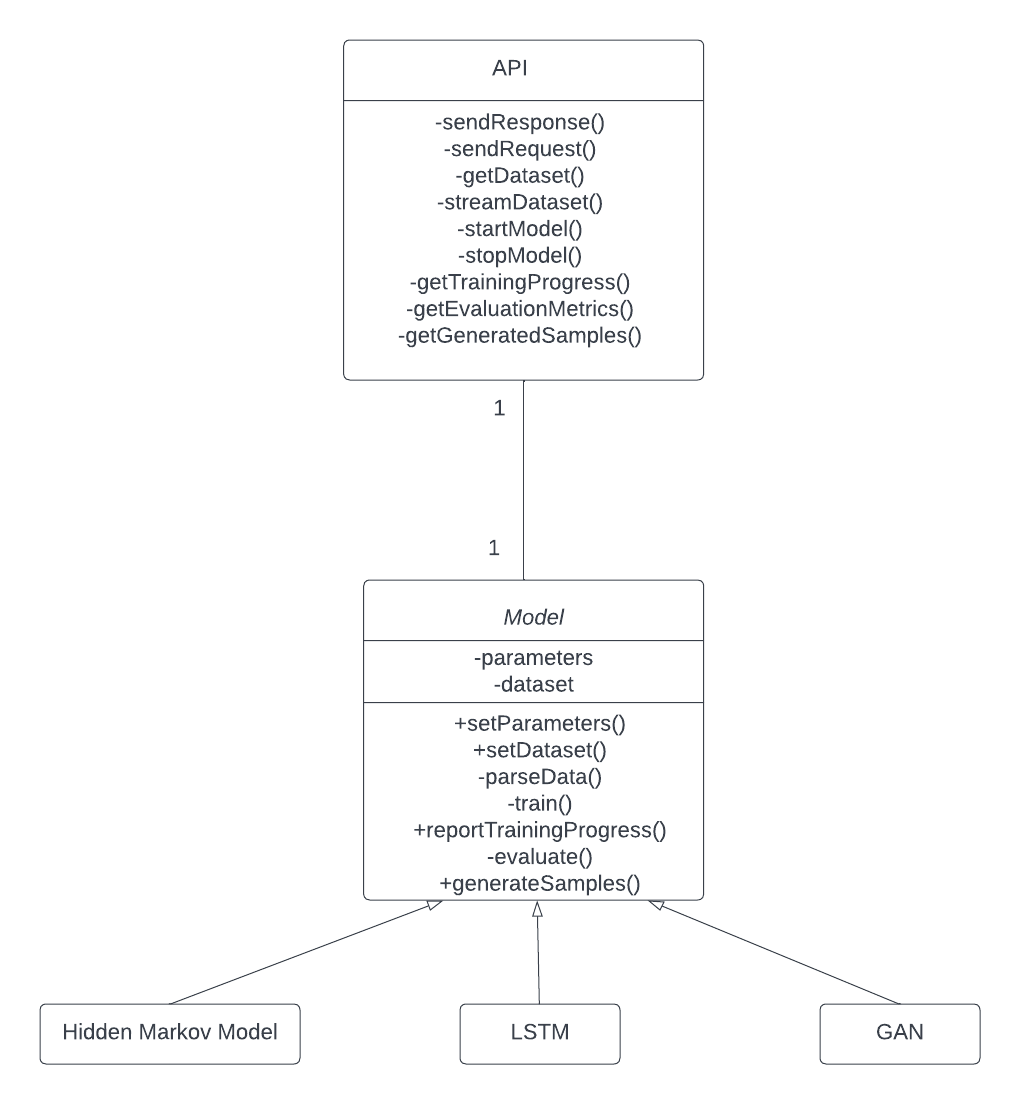
\includegraphics[width=0.7\textwidth]{classdiagram.png}
    \caption{Backend class diagram}
\end{figure}

We define an abstract class \textit{Model}, which then will be implemented by non-abstract classes. These classes will define certain model architecture. They will inherit methods and properties from the \textit{Model} class, so that we can assure that they all are compatible with API (Backend) component. New architectures can be added in an easy way.

Backend component will consist of mainly API endpoint code, that is communication between chosen model and the client, thus it contains only sending and getting information methods. Described in more details in section \ref{sec:communication} and the attached OpenAPI specification (Attach. \ref{att:openapi}).



\section{Communication} \label{sec:communication} % protocols, libraries, network configuration

Our three components have a bidirectional linear communication flow, that is, each component talks with a single other component. Thus we differentiate the following communication schemes:

\subsection{Models \texorpdfstring{$\leftrightarrow$}{<->} Backend}

Since backend and models are just two different Python packages, the communication between them will happen through direct function calls. No special protocol is required here.

\subsection{Backend \texorpdfstring{$\leftrightarrow$}{<->} Frontend}

Here we distinguish two types of communication: request-response and real-time. In both cases the communication can be performed in a unsecure and a secure context. Respectively HTTP/HTTPS and WS/WSS.

\subsubsection{Request-Response}

For single request single response communication we will use the HTTP\footnote{HTTP -- Hypertext transfer protocol} protocol since it is the widely accepted protocol for the web. Our backend will support both HTTP/1.1 and HTTP/2 with the possibility to introduce HTTP/3 support (but not directly implemented by this project). For a meta-protocol REST\footnote{REST -- Representational state transfer} is a popular choice, and thus we will use it but with a small adjustment to adhere to the core CQRS\cite{CQRS}\footnote{CQRS -- Command-Query Responsibility Segregation} principle: queries should be idempotent and fetch some data (represented as HTTP's \texttt{GET} method), commands should modify some data but not return any (represented as HTTP's \texttt{POST} method). This simple modification allows for easier testing and maintainability.

In the attachments (Attach. \ref{att:openapi}) one can find the OpenAPI description of the API.

\subsubsection{Real-Time}

Some aspects will require real-time communication; that is, data can flow both ways without a need for instantiation through requests. For instance, when a model is being trained, backend will have to continuously push data to the frontend client about the current training status. In that case it is unreasonable to expect the client to ask for the newest training status all of the time. WebSockets fit this task perfectly. They allow for creating connections where both ends are able to push messages without any specific trigger.


These can be summarized in a single figure (Fig. \ref{fig:communication-diagram}).

\begin{figure}
    \centering
    
\includegraphics[width=0.7\textwidth]{communication_diagram.png}
    \caption{Communication diagram for all three components. Arrow heads represent the direction of communication.}
    \label{fig:communication-diagram}
\end{figure}

\section{Main components}
% class, states, activity, events diagrams

This section presents state, activity and event diagrams between classes described above.

\subsection{State diagrams}
The only component that will change its state during the runtime is Model class. The model class is initialized at the beginning of the application or when the user decides to train a new model. When the parameters and dataset are selected and the architecture is chosen, the model is ready to be trained. When the user starts to begin the training, the model changes it state to \textit{in training}. Then, the model can be interrupted. An interrupted model can be resumed or deleted. If the model has finished training, it is ready to report evaluation results and generate samples. Then, it can be killed.

This can be summarized by a state diagram as follows:

\begin{figure}[H]
    \centering
    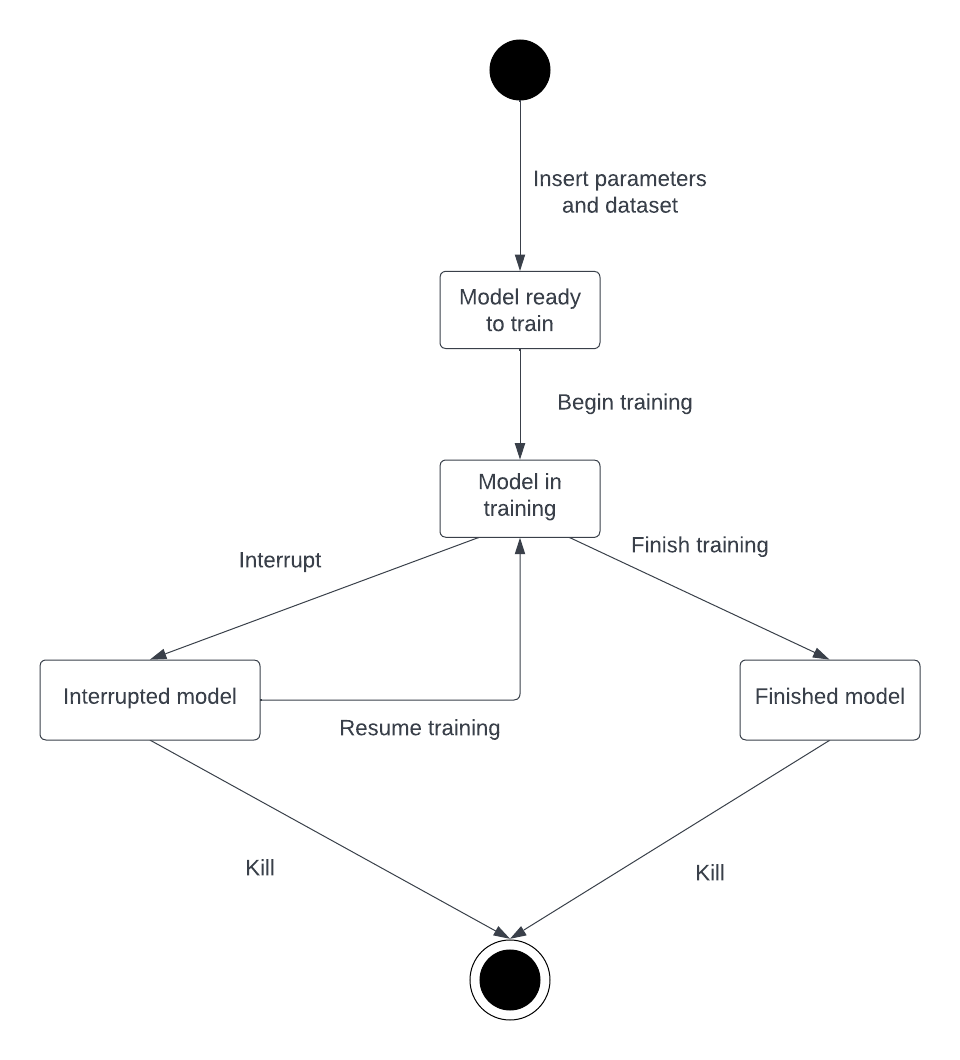
\includegraphics[width=0.7\textwidth]{statediagram.png}
    \caption{State diagram of a model}
\end{figure}

\subsection{Activity diagrams}

As stated before, the application itself has a simple purpose; to enable the user to modify and test an Artificial Intelligence model. Therefore, the activities inside the project are a simple flow of information between the components.

When the user decides to train the model, they select the architecture and parameters. Then, they upload a dataset. The dataset is verified in terms of file format, file size etc. (mentioned in Section \ref{ex_interfaces}). Then, the model begins training. The training can be interrupted by the user and then the user has to decide whether to delete the model or resume training. After the training is finished, the model is evaluated and optionally sample files are generated. According to the user's decision, the model can be saved. Then it is deleted.

\begin{figure}[H]
    \centering
    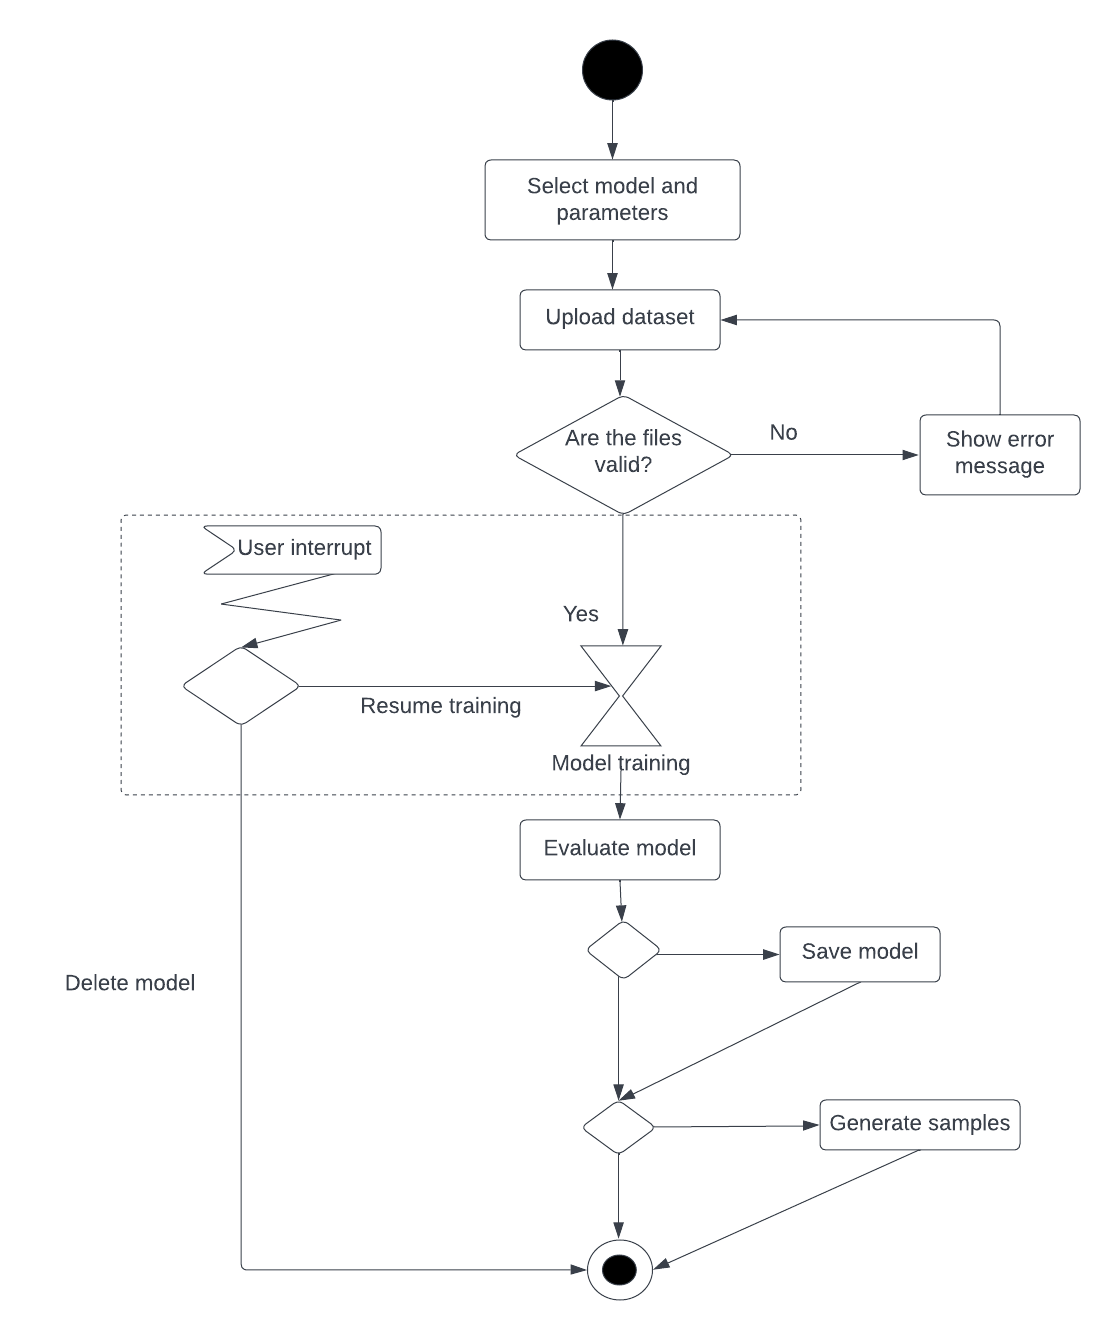
\includegraphics[width=0.8\textwidth]{activitydiagram.png}
    \caption{Activity diagram of custom model training}
\end{figure}

\subsection{Sequence diagrams}

The following diagram illustrates sequential information processing between the user and model. As one can observe, API component is only to forward information between other components.

First, the user configures model and uploads dataset. If the dataset is invalid, model sends a synchronous call that new dataset is required. User must upload a new dataset. This procedure is optional, but can also happen more than once.
Then, the user starts a model. The model repeatedly reports its training progress. Finally, the model reports evaluation metrics. After that, the user can request the model to generate music samples and save the model. These two operations are optional and independent of each other.

\begin{figure}[H]
    \centering
    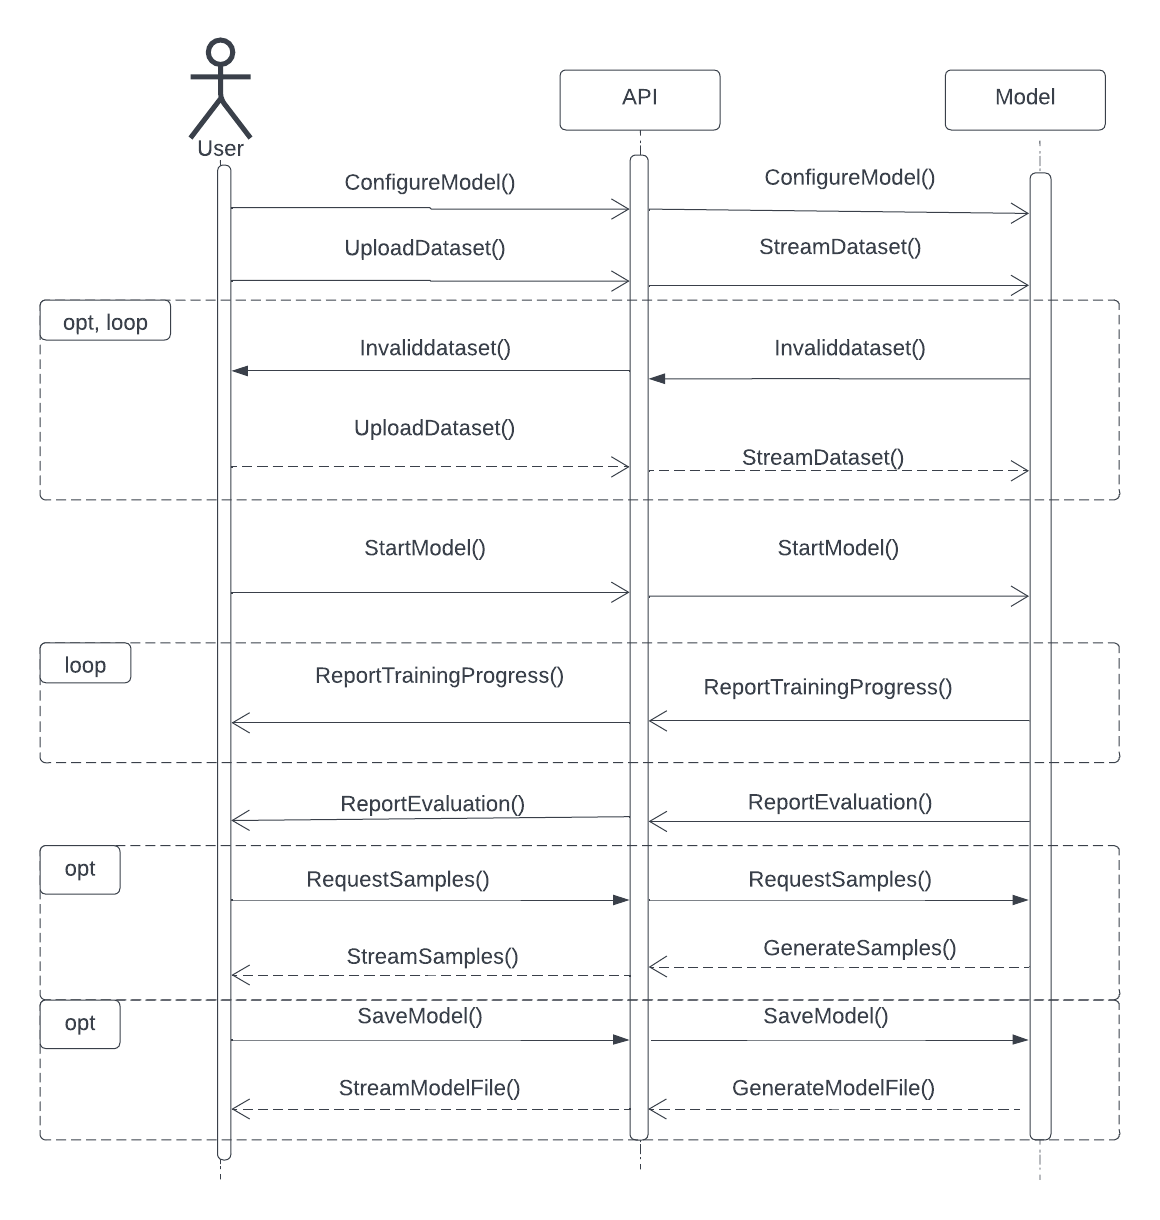
\includegraphics[width=\textwidth]{sequencediagram.png}
    \caption{Sequence diagram of custom model creation}
\end{figure}

\section{GUI vision} % schedules, plots, drawings

The UI will focus on simplicity and ease of use. None of the existing UI frameworks nor design systems suit our needs so we will implement one from scratch in a two-tone design language. The navigation will be linear to have a clear direction of actions to be taken by a user.

The product will follow accessibility principles such as semantic elements, descriptive alt labels, or keyboard navigation. On Fig. \ref{fig:gui_home} we can see two themes supported by the GUI, dark and light. Both have a high contrast which also helps accessibility.

\begin{figure}[H]
    \centering
    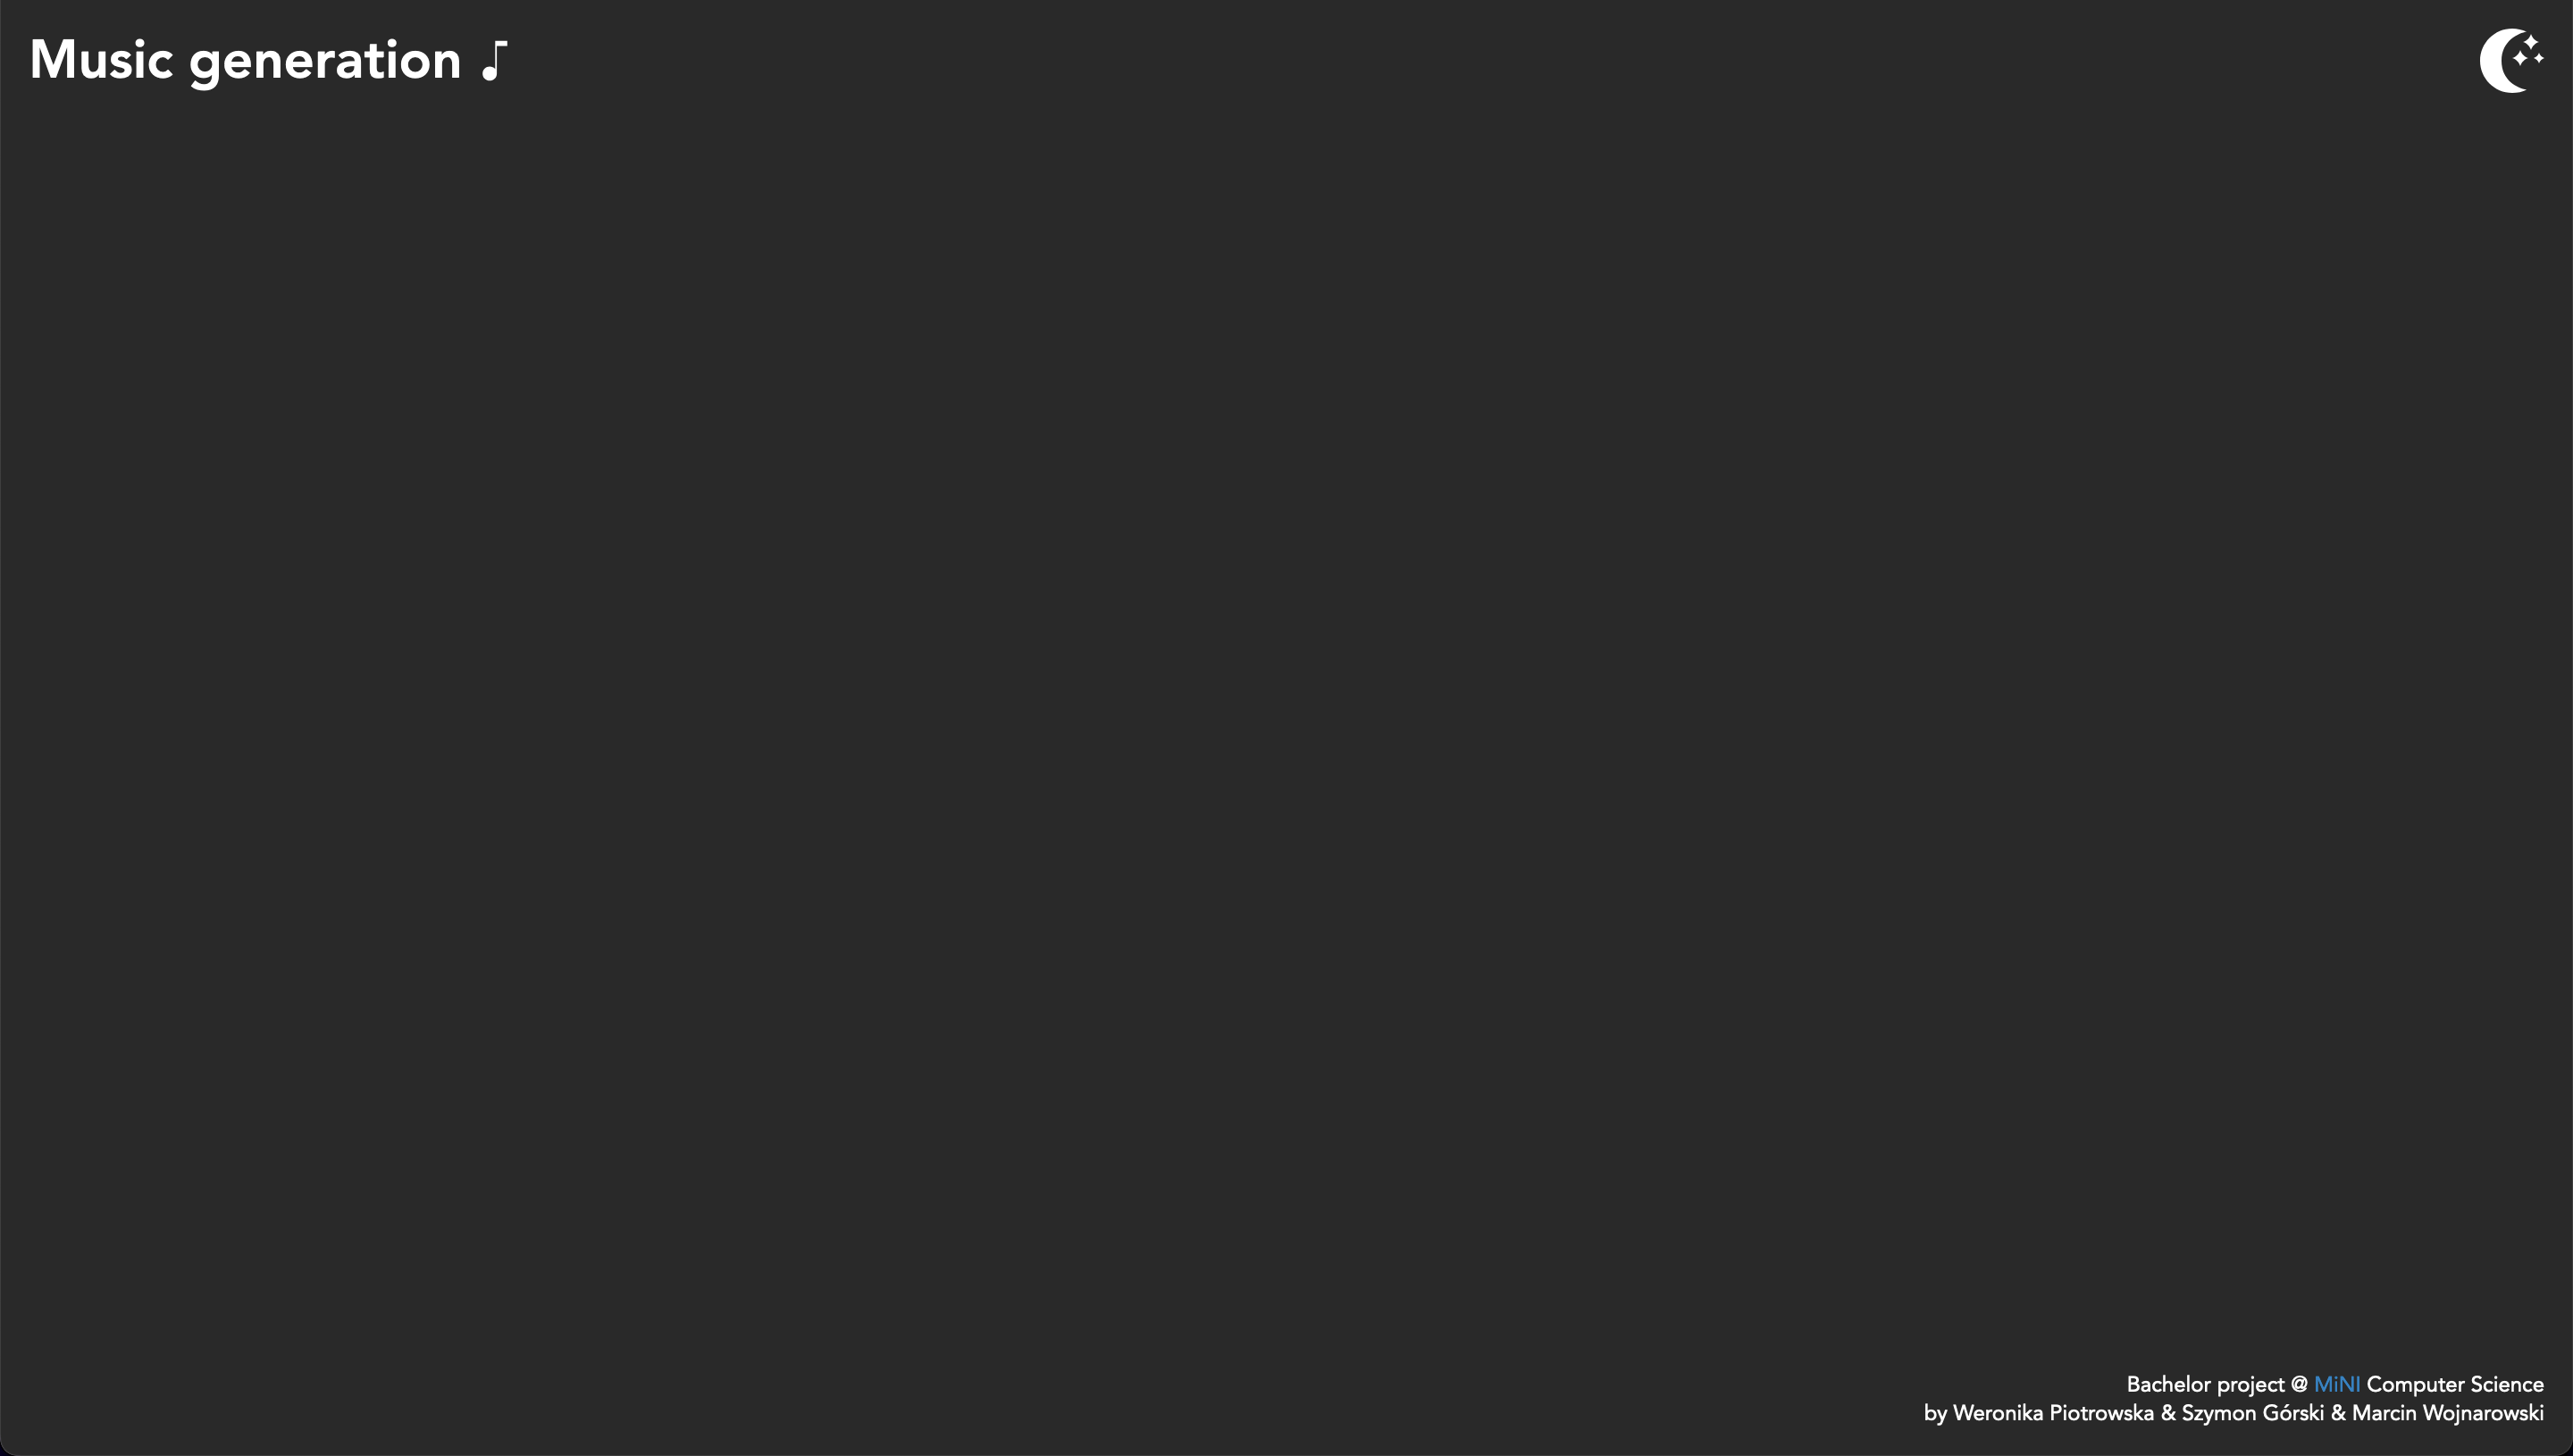
\includegraphics[width=\linewidth]{gui_dark.png}
    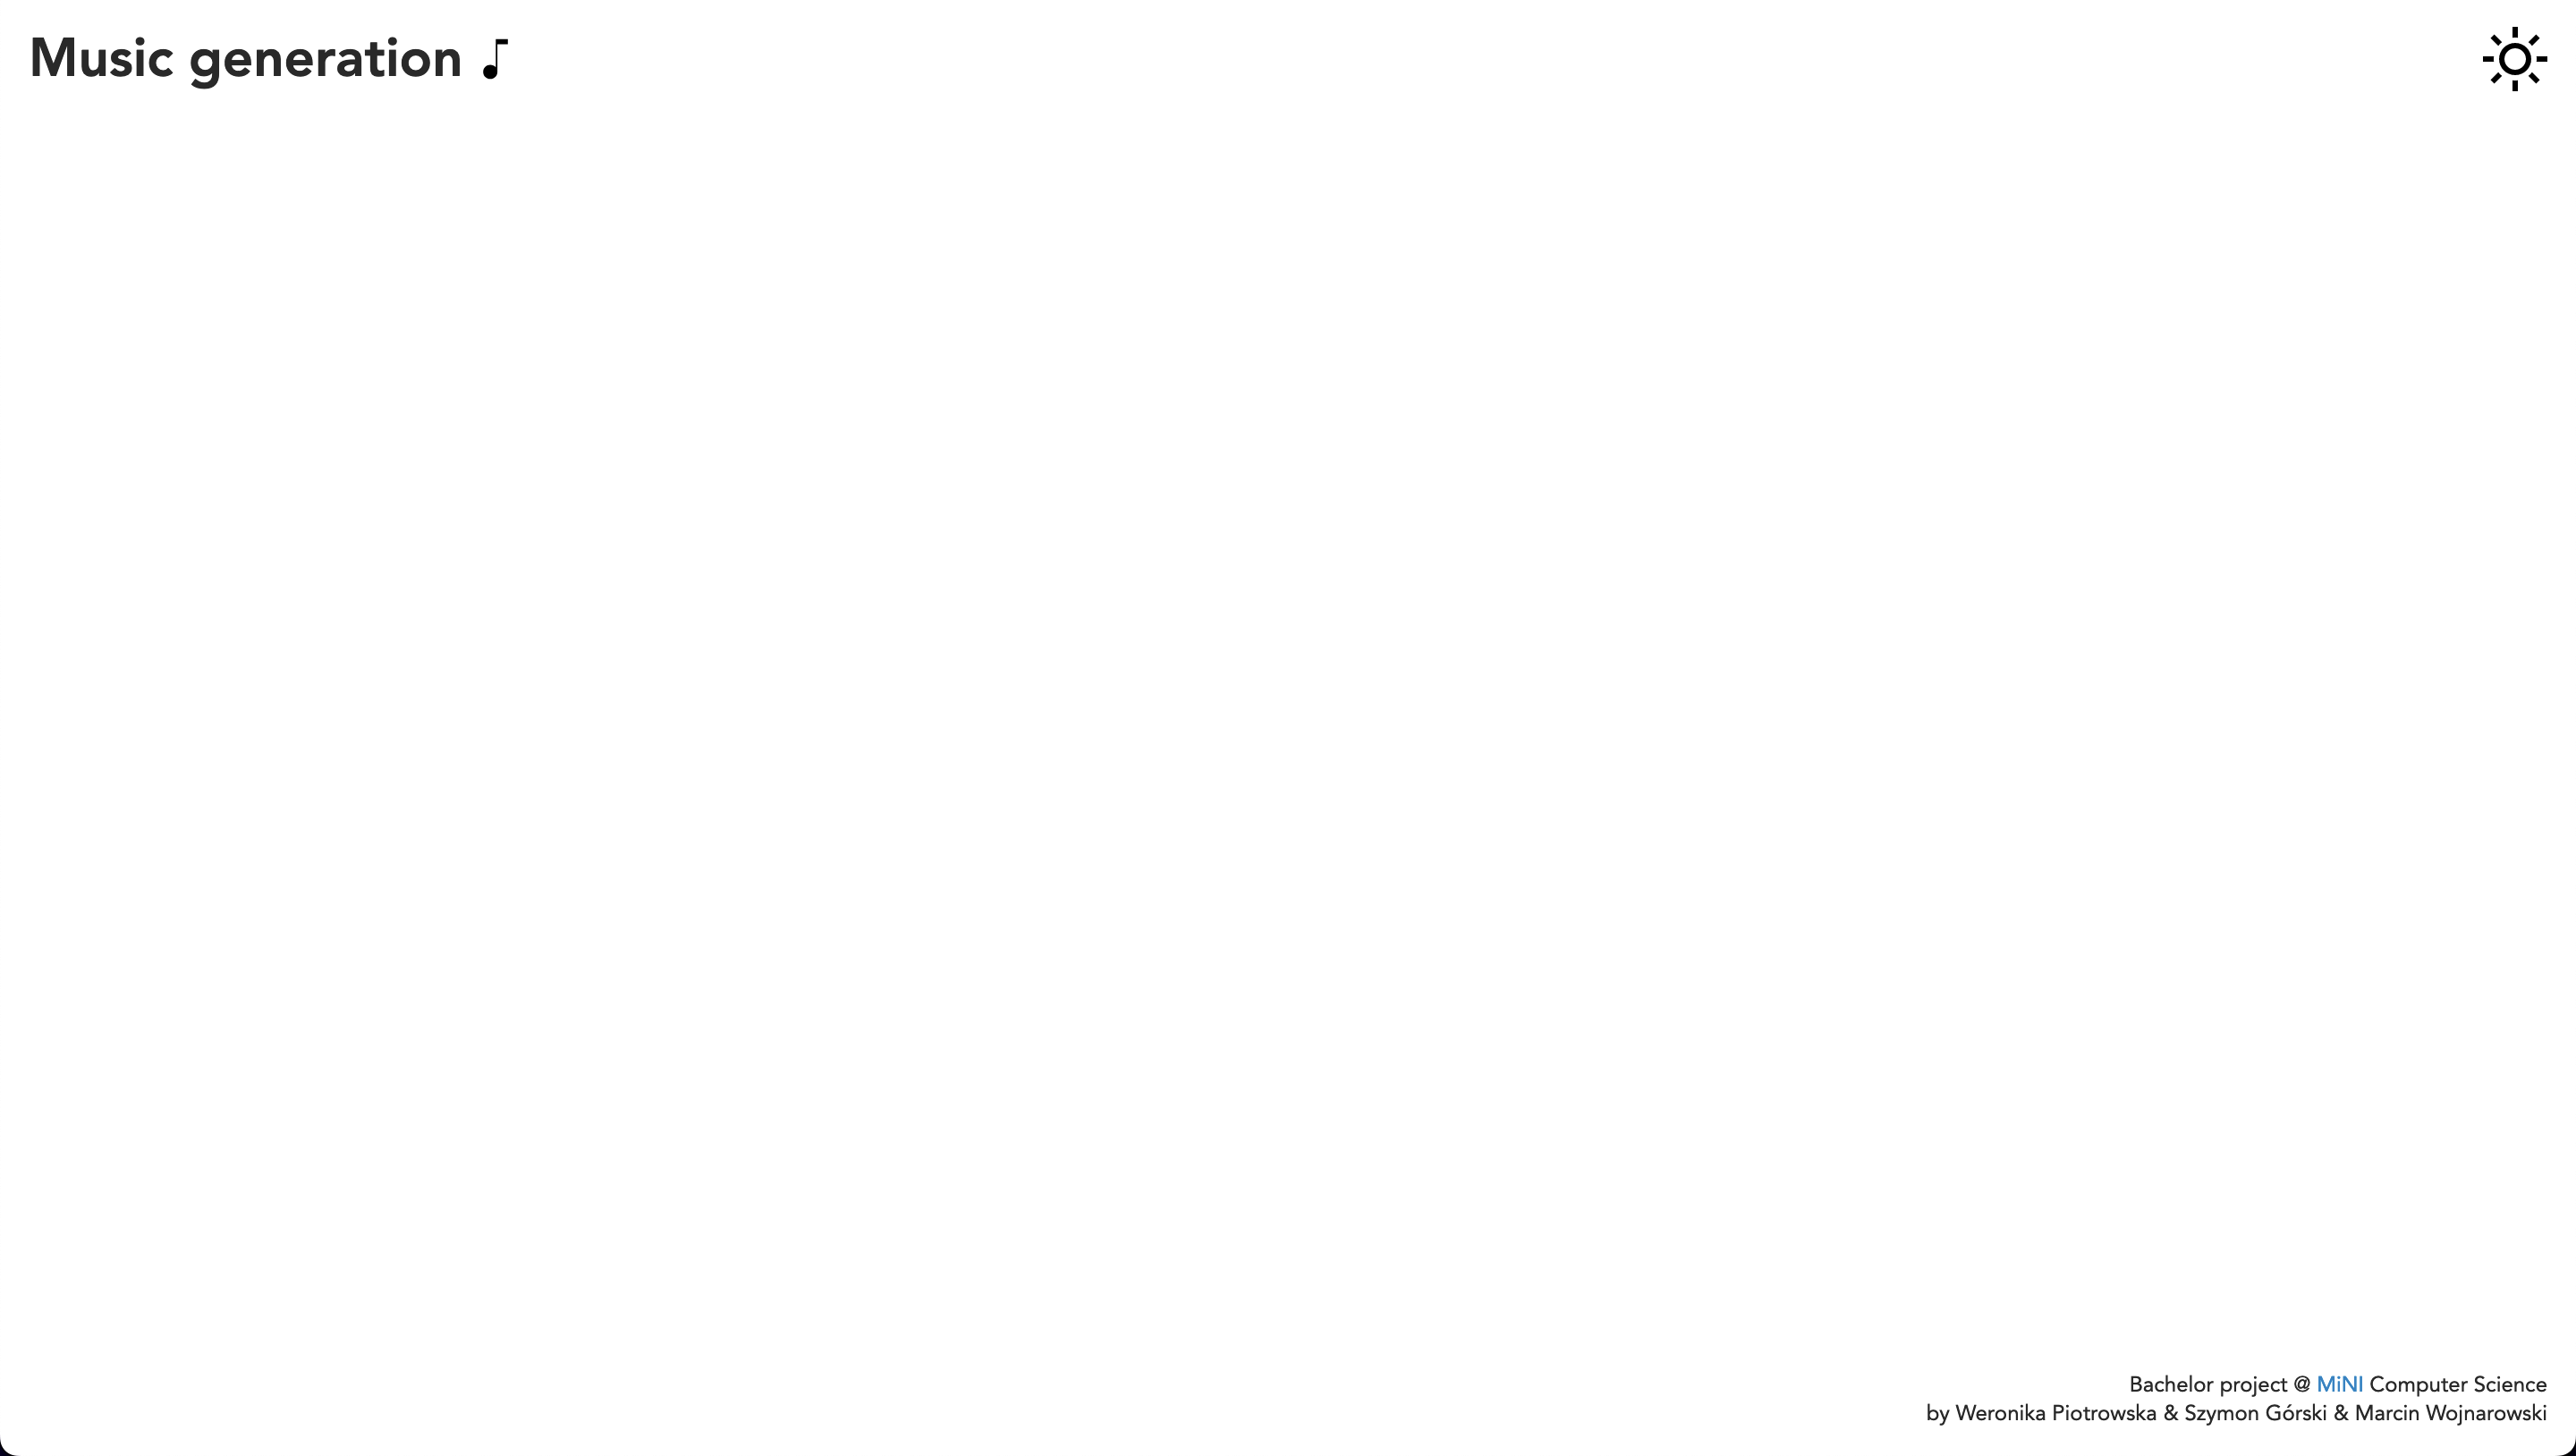
\includegraphics[width=\linewidth]{gui_light.png}
    \caption{Home page of the user interface, in dark and light theme respectively.}
    \label{fig:gui_home}
\end{figure}


To guide the user through the configuration options elements which require an action from the user will be marked with a dashed border (Fig. \ref{fig:gui_action}) but once completed will turn into a solid border.

\begin{figure}[H]
    \centering
    
\includegraphics[width=0.6\linewidth]{gui_action_todo.png}
    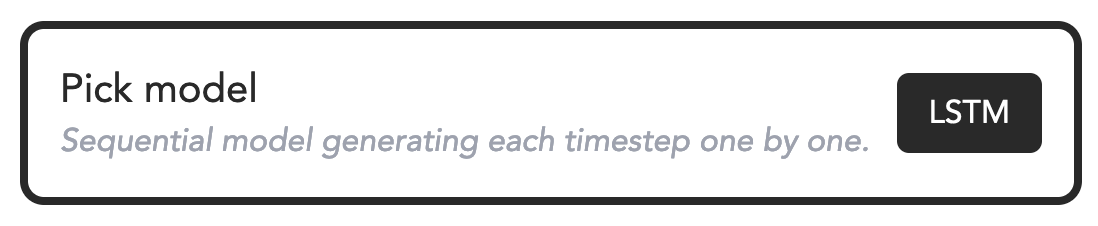
\includegraphics[width=0.6\linewidth]{gui_action_done.png}
    \caption{An element requiring user attention before and after being completed.}
    \label{fig:gui_action}
\end{figure}


During training the UI updates in real-time with training results. These will be represented on a chart and some additional relevant information (Fig. \ref{fig:gui_chart}).

\begin{figure}[H]
    \centering
    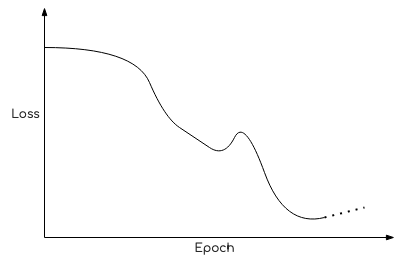
\includegraphics[width=0.5\linewidth]{gui_training_chart.png}
    \caption{Mockup of a live-updating chart with training results. Dotted line represent the currently calculated segment.}
    \label{fig:gui_chart}
\end{figure}

Finally, once training is done user is presented with a possibility of providing a generation seed to generate a larger sample of music. To do this input will be accepted both from user's keyboard and an on-screen piano keyboard. After a seed is recorded it can be played back by the user to be verified for correctness (Fig. \ref{fig:gui_record_seed}).

\begin{figure}[H]
    \centering
    
\includegraphics[width=0.4\linewidth]{gui_record_seed.png}
    \caption{Mockup of a on-screen piano keyboard for recording a seed.}
    \label{fig:gui_record_seed}
\end{figure}

\section{External interfaces} \label{ex_interfaces} % standards, file formats, norms

The only external interface we will be using is when uploading and downloading files. User's own dataset must be uploaded as a set of \texttt{.midi} or \texttt{.mid} files and cannot weigh more than 10MB. Each uploaded file must not weigh more than 500KB. For comparison, the entire initial training dataset weighs 3MB. Additionally, we do not allow files to be in folders and they must not be password protected. The maximum length of filename is 64 characters.

All files will be asserted to be correct in above conditions before running the model. Filename changes may be applied before further processing.


\section{Technology selection} % languages, libraries, platforms, OS

Our goal is to be as cross-platform as possible. That is why our selection of technologies focuses on solutions which give us the possibility to abstract over the underlying platform. Arguably nowadays the most ubiquitous platform is web. That is why our frontend will be built for the web platform using standard cross-browser features.

The frontend will consist of a client-side-rendered web page distributed as a set of static JS, CSS, and HTML files. To build these files the \href{https://www.typescriptlang.org/}{Typescript} language will be used, as it provides static types to the inherently dynamic Javascript which will be useful for development. To build the HTML DOM a UI library named \href{https://reactjs.org/}{React} will be used because it gives an unopinionated and simple approach to building user interfaces. For CSS \href{https://tailwindcss.com/}{Tailwind} will be used, but the styling will be custom. All variants of testing (unit, integration) will be performed with the use of \href{https://vitest.dev/}{Vitest} which is a more modern alternative to (but compatible with) \href{https://jestjs.io/}{Jest}. Finally, for building the final output \href{https://vitejs.dev/}{Vite} is used as it provides the best developer experience and fast development cycle. We plan to use modern and ECMAScript\footnote{ECMAScript -- Standard defining what is commonly known as Javascript}-compliant web APIs to be able to target any platform which has a web browser.

The backend will be written in \href{https://www.python.org/}{Python} for a single, simple reason: our models are written in Python. Shortcomings of Python as a web server are well understood by us, but we made an executive decision to use the same language for both the models and backend to greatly simplify their communication (it will result in a direct function call, instead of an additional communication layer). Given that, we chose \href{https://fastapi.tiangolo.com/}{FastAPI} for creating HTTP and WebSocket APIs. For testing the built-in \texttt{unittest} package and FastAPI's functions will be used. For a better static verifiability Python type hints will be used. Any platform with a Python interpreter will be able to run this web server, given that the dependencies of the models can be resolved.

Which brings us to the final component; the models themselves. These will be written in Python due to it being the go-to language for machine learning. Most machine learning libraries target Python, out of a crowd of candidates we are going with \href{https://www.tensorflow.org/}{Tensorflow} due to its large community support and seamless GPU/CPU interchangeability. There exist CUDA, Metal, JS, WebGL, and NumPy backends for Tensorflow, so our code should work on any platform these backends can run on.

Finally, to ease deployment \href{https://www.docker.com/}{Docker} will be used to be able to spin up the whole project in a sandboxed environment with a single command.

\newpage
\section{Attachments}

\begin{enumerate}
    \item \label{att:openapi} The OpenAPI description of the HTTP API
\end{enumerate}


\printbibliography


\end{document}
